\documentclass[11pt]{article}
\usepackage[letterpaper,margin=1in]{geometry}
\usepackage[T1]{fontenc}
\usepackage{mathptmx}
\usepackage{amsmath,amssymb}
\usepackage{graphicx}
\usepackage{booktabs}
\usepackage[font=small,labelfont=bf]{caption}
\usepackage[numbers,sort&compress]{natbib}
\usepackage{xcolor}
\usepackage{microtype}
\usepackage{authblk}
\usepackage[colorlinks=true,linkcolor=blue!50!black,citecolor=blue!50!black,urlcolor=blue!50!black]{hyperref}
\setlength{\emergencystretch}{3em}
\renewcommand{\baselinestretch}{1.12}

\title{Dipoles of nonparabolic quantum-well states: why orthonormalizing the bound states is not enough}
\author{Gracen Ownby}
\affil{University of Oklahoma, Norman, Oklahoma, USA}
\date{\small 20 October 2026}

\begin{document}
\maketitle

\begin{abstract}
Intersubband dipole matrix elements are routinely computed from the one-band Schr\"odinger equation with an energy-dependent effective mass. Its eigenstates belong to different Hamiltonians and are not orthonormal in the ordinary inner product. They are orthonormal only as two-component states of the two-band Kane model from which the energy-dependent mass derives, and the dipole of two such states contains a light-particle term besides the conduction one. We compare common procedures with the two-band dipoles for three InGaAs/InAlAs structures in boxes of 100--800~\AA\ of barrier, at fixed potentials so that only the box changes. Without orthogonalization the dipoles are off by 2--8\% and depend on the coordinate origin. Using the two-band norm without the light-particle term is worse (5--14\%). Gram--Schmidt or L\"owdin orthonormalization of the bound states cannot correct the norm: the dipole of a single well is 4.9\% too large although its two states are orthogonal by parity. L\"owdin orthonormalization of the bound states alone corrects the lower dipoles to 0.4\% but leaves those of the topmost bound state 5--7\% wrong in every box, and the peak second-order susceptibility of a double well 9\% too large; a first-order expansion shows that the top state lacks its orthogonalization partners above. Including all box states within 0.5~eV above the bound ones brings every dipole within 0.8\% of the two-band value; a fixed small number of extra states does not, because the energy it spans shrinks as the box grows. Even a complete one-band L\"owdin basis leaves a residual of 0.3--0.5\%, which shrinks to 0.2\% when $\hslash^2E_g/2m^*$ is made uniform, so the orthonormalized one-band dipoles converge to a limit of their own. The two-band dipoles are exact within the model, need no extra states and cost one derivative per state.
\end{abstract}

\section{Introduction}
Most calculations of intersubband (ISB) absorption, quantum-cascade transport and ISB nonlinear optics in narrow-gap quantum wells use a one-band envelope equation in which the effective mass depends on energy \cite{Nelson1987,Ekenberg1989,Sirtori1994,JirauschekKubis2014},
\begin{equation}
-\frac{d}{dz}\frac{\hslash^2}{2m(E,z)}\frac{d\psi}{dz}+V(z)\psi=E\psi,\qquad m(E,z)=m^*(z)\left[1+\frac{E-V(z)}{E_g(z)}\right].
\label{eq:H}
\end{equation}
The eigenproblem is nonlinear in $E$. Each eigenvalue belongs to its own Hamiltonian $H(E)$, so eigenstates of different energy are not orthogonal in the ordinary inner product \cite{JirauschekKubis2014,Jonasson2016,Mohamed2024}. The equation derives from a two-band Kane model, in which each state has a light-particle component
\begin{equation}
\phi_n(z)=\sqrt{\frac{\hslash^2E_g}{2m^*}}\,\frac{\psi_n'(z)}{E_n-V(z)+E_g}.
\label{eq:phi}
\end{equation}
The two-component states are orthogonal, $\int(\psi_m\psi_n+\phi_m\phi_n)\,dz=N_n\delta_{mn}$ \cite{Sirtori1994,Mohamed2024}, and the norm is the general one for energy-dependent Hamiltonians, $N_n=\langle\psi_n|1-\partial H/\partial E|\psi_n\rangle$ \cite{Formanek2004}. Their dipoles are
\begin{equation}
z^K_{mn}=\frac{\int(\psi_m z\psi_n+\phi_m z\phi_n)\,dz}{\sqrt{N_mN_n}} .
\label{eq:zK}
\end{equation}
The light-particle weight $\int\phi_n^2dz$ is 6--22\% of the conduction weight for the states considered here.

Codes handle the overlap of the one-band states in different ways. Some use the two-band (or three-band) states \cite{Mohamed2024}, some avoid the energy-dependent mass in the growth direction \cite{Jonasson2016}, and many ignore the overlap or orthonormalize the bound states, by Gram--Schmidt or by L\"owdin's symmetric orthonormalization \cite{Lowdin1950}, which changes the states least in the least-squares sense \cite{CarlsonKeller1957}. Imam \emph{et al.} quantified the overlaps that remain for quasi-bound states \cite{Imam2000}. That a symmetric orthonormalization depends on where the set is truncated is known in quantum chemistry; how large the effect is for ISB dipoles, and what it does to nonlinear susceptibilities, has to our knowledge not been reported. We came across it while auditing calculations of ISB second-order nonlinearities, where L\"owdin orthonormalization of the bound states made one susceptibility 9\% too large. Here we separate the errors of the common procedures and give a rule.

\section{Method}
We solve Eq.~\eqref{eq:H} for In$_{0.53}$Ga$_{0.47}$As wells ($m^*=0.043\,m_0$, $E_g=0.75$~eV) and In$_{0.52}$Al$_{0.48}$As barriers ($0.075\,m_0$, 1.45~eV, offset 0.52~eV) on a 0.5~\AA\ grid, with hard walls at the ends of a barrier padding of 100--800~\AA\ (half on each side), using qwkit \cite{qwkit}. The structures are:
\begin{itemize}
\item a 64/10/29~\AA\ asymmetric double well at zero field (three bound states);
\item a 58/14/34/14/58~\AA\ triple well at 55~kV/cm (five);
\item a 60~\AA\ single well at zero field (two).
\end{itemize}
The potentials are fixed (not self-consistent), so that changing the padding changes only the box. States count as bound if they lie below the lower barrier edge next to the wells and have at least 80\% of their probability within 25~\AA\ of the wells; resonances above the barrier are excluded however localized they appear in a small box. 120 states are solved.

The light-particle component, Eq.~\eqref{eq:phi}, is discretized exactly as the solver discretizes $H(E)$. On each half point the mass is the mean of the node masses, $m_h(E)=A_h+B_hE$, and $\phi_h=\sqrt{\hslash^2B_h/2}\,(\psi_{i+1}-\psi_i)/(m_h(E)\,\Delta z)$, with one extra point at each wall. The product $\phi_m\phi_n$ is then the divided difference of the discrete $H(E)$ between $E_m$ and $E_n$, and the two-component overlaps vanish to $3\times10^{-13}$. We compare, against $z^K_{mn}$ of Eq.~\eqref{eq:zK}:
\begin{itemize}
\item \emph{raw}: normalized one-band states without orthogonalization (origin at the centre of the wells);
\item \emph{norm only}: the two-band norm $N_n$ without the light-particle dipole term;
\item \emph{GS}: Gram--Schmidt of the bound states from the lowest up;
\item \emph{L-bound}: L\"owdin orthonormalization of the bound states, $\tilde\Psi=\Psi S^{-1/2}$ with $S=\Psi^T\Psi$;
\item \emph{L-buffer}: L\"owdin orthonormalization of the bound states together with the next 2 or 10 box states, with all box states up to 0.5, 1 or 2~eV above the topmost bound state, or with all 120 states, then truncated to the bound states.
\end{itemize}
We report relative errors of all allowed dipoles between the lowest four bound states, and of the peak second-order susceptibility for second-harmonic generation through the lowest three states (linewidth 10~meV).

\section{Results}
Figure~\ref{fig:err} shows the largest dipole error of each procedure against the box size, and Table~\ref{tab:err} lists the largest errors.

\emph{Raw states and the norm.} The one-band overlaps between bound states reach 0.025. Without orthogonalization the dipoles are off by 1.8--5.6\% (double well), 1.8--8.0\% (triple well) and 4.9\% (single well), and the peak susceptibility of the double well by 10\%. Raw dipoles also depend on the origin of $z$, since $\langle m|z+a|n\rangle=z_{mn}+aS_{mn}$: moving the origin by 100~\AA\ changes the largest error to 16\% (double well) and 26\% (triple well). The single well isolates the norm. Its two bound states have opposite parity and are exactly orthogonal, yet $z_{12}$ is 4.9\% too large, with or without orthogonalization of the bound states, which does nothing here. The one-band norm omits the light-particle weight, which is larger for the excited state, and the light-particle components carry their own dipole. Applying only the two-band norm is worse than nothing: the dipoles come out 5--14\% too small, and the susceptibilities 20--23\% too small, because the light-particle dipole term, of the same order, is missing. Gram--Schmidt leaves errors of up to 3.9\% (double well), 5.0\% (triple well) and 4.9\% (single well), and its result depends on the order of the states.

\emph{Truncation.} L\"owdin orthonormalization of the bound states corrects the dipoles among the lower states to within 0.4\% but not those of the topmost bound state: $z_{13}$ and $z_{23}$ of the double well are 6.8\% and 2.3\% too large, $z_{14}$ of the triple well 5.4\%, and the peak susceptibility of the double well comes out 8.9--9.1\% too large. At fixed potential these errors do not change with the box (100--800~\AA), because they are set by the bound states. Expanding $S^{-1/2}=1-\tfrac12D+O(D^2)$ with $D=S-1$,
\begin{equation}
\tilde z_{mn}\approx z_{mn}-\tfrac12\sum_{k\in\mathcal B}\left(S_{mk}z_{kn}+z_{mk}S_{kn}\right),
\label{eq:first}
\end{equation}
with $\mathcal B$ the set orthonormalized, reproduces the L-bound errors to 0.2 percentage points. For a state in the middle of the set, its overlaps with the states above and below enter with their dipoles. For the topmost state, the partners above it are missing from $\mathcal B$, and because the dipoles to the next states up are the largest, the omission is not small. Extending the sum in Eq.~\eqref{eq:first} to all 120 states brings the errors of the top-state dipoles from 5--7\% to 0.5--1.9\% (the remainder is of second order in the overlaps), so the artefact comes mostly from the missing partners. Where the line between bound and unbound states is drawn is a choice; a resonance just above the barrier that is counted as bound in a small box changes the L-bound result abruptly.

\emph{Buffers.} Including box states above the bound ones restores the missing partners. A buffer of all states within 0.5~eV above the topmost bound state brings every allowed dipole within 0.76\% of the two-band value in all structures and boxes, and the peak susceptibility within 1.0\%; 1~eV gives 0.55\%. A buffer of a fixed number of states is unreliable, because the energy it spans shrinks as the box grows. Two extra states give at most 0.8\% in the 100~\AA\ box but 4.7--5.8\% at 800~\AA, and even ten extra states reach 1.4\% for the single well at 800~\AA, where they span only 0.26~eV.

\emph{The limit of L\"owdin.} The buffered dipoles do not converge to the two-band ones. With all 120 states the residual is 0.25--0.49\% (double well), 0.35\% (triple well) and 0.26--0.41\% (single well), and it does not shrink with a larger buffer. L\"owdin over a complete one-band set is an orthogonal transformation of the grid basis, so its position matrix has the grid points as eigenvalues. The two-band position matrix of Eq.~\eqref{eq:zK} is instead the conduction block of a two-component operator. To first order in the light-particle components, the two agree only if $\phi_n$ is a position- and energy-independent multiple of $\psi_n'$. In the structures here $K=\hslash^2E_g/2m^*$ differs between well and barrier (it is 66.5 and 73.7~eV\,\AA$^2$); choosing the barrier gap to make $K$ uniform reduces the residual to 0.16--0.26\%, and the 0.5~eV buffer then agrees with the two-band dipoles to 0.12\%. The rest comes from the energy dependence of Eq.~\eqref{eq:phi}.

\begin{figure}[t]
\centering
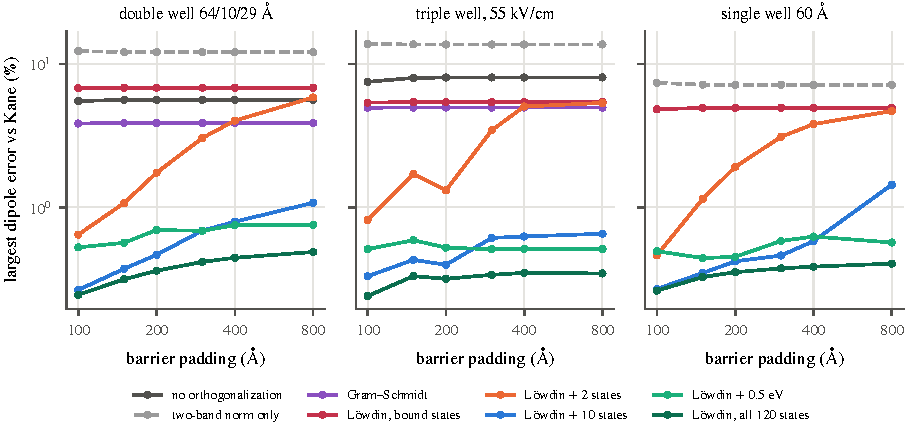
\includegraphics[width=\textwidth]{figures/fig1_errors.pdf}
\caption{Largest relative error of the allowed dipoles between the lowest four bound states against the two-band dipoles, as a function of the barrier padding, at fixed potential.}
\label{fig:err}
\end{figure}

\begin{table}[t]
\centering
\small
\caption{Largest relative dipole error (\%) against the two-band dipoles over all allowed transitions among the lowest four bound states and paddings of 100--800~\AA, and the peak second-order susceptibility error of the double well.}
\label{tab:err}
\begin{tabular}{lcccc}
\toprule
Procedure & double well & triple well, 55 kV/cm & single well & $\chi^{(2)}$, double well \\
\midrule
raw & 5.6 & 8.0 & 4.9 & $+10$ \\
two-band norm only & 12.3 & 13.7 & 7.4 & $-23$ \\
Gram--Schmidt & 3.9 & 5.0 & 4.9 & $+8.2$ \\
L\"owdin, bound states & 6.8 & 5.4 & 4.9 & $+9.1$ \\
L\"owdin + 2 states & 5.8 & 5.4 & 4.7 & $+0.7$ to $+7.8$ \\
L\"owdin + 10 states & 1.1 & 0.7 & 1.4 & $+0.4$ to $+1.9$ \\
L\"owdin + 0.5 eV & 0.8 & 0.6 & 0.6 & $+0.7$ to $+1.0$ \\
L\"owdin + 1 eV & 0.6 & 0.4 & 0.5 & $+0.4$ to $+0.7$ \\
L\"owdin, all 120 states & 0.5 & 0.4 & 0.4 & $+0.4$ to $+0.7$ \\
\bottomrule
\end{tabular}
\end{table}

\section{Recommendation}
\begin{itemize}
\item Use the two-band dipoles, Eq.~\eqref{eq:zK}: both the norm and the light-particle dipole term, with $\phi_n$ discretized consistently with the solver. They are exact within the model, need no states beyond those of interest and cost one derivative per state, as Mohamed \emph{et al.} also recommend for quantum-cascade levels \cite{Mohamed2024}. Their orthogonality is a check of the eigensolver.
\item Never apply the two-band norm without the light-particle dipole term.
\item If a code must orthonormalize one-band states, do it over the bound states and all box states within at least 0.5~eV above them, never over the bound states alone, and not with a fixed small number of extra states. Expect a residual of a few tenths of a per cent.
\item Raw one-band dipoles depend on the coordinate origin and should not be used.
\end{itemize}
The errors matter most where the topmost bound state takes part: second-order nonlinearities of double-resonance designs, in which the third state is often the topmost bound one, and weak transitions. For the double well studied here, the susceptibility error of L\"owdin over the bound states (9\%) exceeds typical design tolerances. Because the topmost state changes when a state binds or unbinds, design optimizations or uncertainty analyses that cross such a point see a spurious jump.

The calculations are in one material system, with the two-band form of $m(E)$. Codes that use a three-band $m(E)$ \cite{Sirtori1994} need the corresponding light-particle components, but the separation into a norm error and a truncation error is general. qwkit up to version 0.6.0 orthonormalized the bound states alone; version 0.6.1 adds a fixed buffer of ten states, which spans more than 0.5~eV in the 200~\AA\ boxes of our earlier calculations, and version 0.6.2 adds an energy buffer and the exact discrete two-band partner.

\section{Conclusion}
One-band dipoles of nonparabolic quantum-well states carry two distinct errors. A norm-and-light-particle error of a few per cent cannot be removed by orthogonalizing the bound states among themselves. When L\"owdin orthonormalization is restricted to the bound states, a truncation error of 5--7\% appears in the dipoles of the topmost bound state. The two-band dipoles remove both exactly. A L\"owdin buffer of 0.5~eV of box states removes them to below 1\%, but converges to a limit that differs from the two-band dipoles by a few tenths of a per cent.

\section*{Data and code availability}
The \texttt{qwkit} software package (v0.7.0) is archived at \url{https://doi.org/10.5281/zenodo.23444120}. The simulation scripts, raw JSON datasets, and figure-generation code that reproduce every result in this study are permanently archived at \url{https://doi.org/10.5281/zenodo.23444554}.

\bibliographystyle{unsrtnat}
\bibliography{refs}
\end{document}
